\chapter{Architektur Konzept}
In diesem Kapitel wird die Struktur und Architektur des Hardware-Health-Monitroing Lösung erläutert. Die Architektur wird dabei zur Übersichltichkeit in drei hauptkomponenten unterteilt.\\
Abschnitt \ref{sec:Datenerfassung} befasst sich dabei mit der Datenerfassung. Hier wird das Konzept zum Plattform übergreifenden Auslesen der Hardwaresensorik und der Schpeicherung der erfasten Messdaten beleuchtet. In Abschnitt \ref{sec:Datenverarbeitung} wir anschließend das Modell zur bewertung des Systemzustnads erläutert. Das Konzept zur Visualisierung der Daten wird anschließend in \ref{sec:Datenvisualisierung} beleuchtet. Zuletzt werden die Teilsysteme in Abschnitt \ref{sec:Gesamtkonzept} zu einem Gesamtsystem zusammengeführt. 

\section{Datenerfassung}\label{sec:Datenerfassung}
Bla bla bla
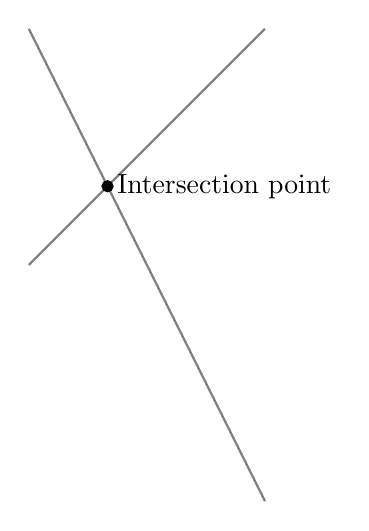
\begin{tikzpicture}
    \draw[gray, thick] (-1,2) -- (2,-4);
    \draw[gray, thick] (-1,-1) -- (2,2);
    \filldraw[black] (0,0) circle (2pt) node[anchor=west]{Intersection point};
    \end{tikzpicture}
\subsection{Entwurf einer Architektur zum Auslesen der Systemhardware}
\subsection{Entwurf eines Datenbankmodells zum Speichern der Messwerte}

\section{Datenverarbeitung}\label{sec:Datenverarbeitung}
\subsection{Health Status Definition}
\subsection{Ermittelung des Health Status}
\subsection{Ermittelung der Systemstatus Historie}
\subsection{Ermittelung der Systemzuverlässigkeit}

\section{Dashboard}\label{sec:Datenvisualisierung}
\subsection{Bereitstellung der Daten}
\subsection{Konzeptentwurf zur Datenvisualisierung}

\section{Entwurf eines Task Scheduling Verfahrens}\label{sec:Gesamtkonzept}

\chapter{Prototypische Implementierung}

\section{Implementierung des Taskschedulers}

\section{Implementierung einer Plattform unabhängigen Datenerfassung}
\subsection{Umsetzung der Hardware Services}
\subsection{Umsetzung der Datenbank Services}
\subsection{Umsetzung der Strategien zur Datenerfassung}

\section{Implementierung der Datenverarbeitung}
\subsection{Implementierung der Algorithmen zur Health Status Erfassung}

\section{Implementierung der Datenvisualisierung}
\subsection{Implementierung der API}
\subsection{Aufbau eines Dashboards}


\chapter{Ausblick}